\section{Introduzione}
Il nostro progetto consiste nella realizzazione di un content-based recommender system che raccomandi item rappresentando gli oggetti e le preferenze degli utenti sfruttando i dati provenienti dalla Linked Open Data Cloud al fine di poter aumentare l'efficienza del recommender system utilizzando informazioni aggiuntive inerenti un particolare film utilizzando differenti fonti.

\subsection{Open Data e Linked Data}
L’interoperabilità è uno dei vantaggi più importanti del modello Open Data. I dati, se isolati, hanno poco valore; viceversa, il loro valore aumenta quando data set differenti, prodotti e pubblicati in modo indipendente da diversi soggetti, possono essere incrociati fondendo e integrando le informazioni. Questo è alla base del processo di creazione di valore aggiunto sui dati: le applicazioni. Le applicazioni, di valore sociale e/o economico, sfruttano quello che può essere visto come un grande database aperto e distribuito per offrire viste e servizi. L’interoperabilità è dunque un elemento chiave di uno degli aspetti più innovativi offerti dagli Open Data: l’uso dei dati in modi e per scopi “inattesi”, nuovi in quanto non previsti dai singoli enti e dai  soggetti che pubblicano i “dati grezzi”.

Per consentire il riuso dei dati occorre poter combinare e mescolare liberamente i dataset. Occorre cioè collegare i dati tra loro, stabilendo un link diretto quando i dati (possibilmente provenienti da diverse sorgenti) si riferiscono a oggetti identici o comunque relazionati tra loro. Tale collegamento diretto si manifesta come la possibilità di “saltare” da un dataset all’altro, ad esempio quando si vuole accedere a dati (come i dettagli su una particolare entità) che non si posseggono al’interno.
Supponiamo per esempio di avere, da una parte, amministrazioni locali che pubblicano dati aperti relativi ai monumenti storici e agli hotel che si trovano nelle vicinanze di quei monumenti; dall’altra, Sovrintendenze ai Beni Culturali che pubblicano dati dettagliati sui monumenti, gli artisti e i periodi storici, e sui quadri esposti nei musei o nei palazzi.
Combinare i due dataset potrebbe essere di grande utilità, ad esempio per offrire un servizio personalizzato sugli itinerari in base agli interessi culturali specifici di un turista.
Per fare questo, se i dati non sono “collegati” (linked) occorre in qualche modo creare questi link, processando i dati a mano o attraverso algoritmi ad hoc. Questo processo può non essere banale e sicuramente è una barriera al riuso organico dei dati.

Nei cosiddetti Linked Data, questi collegamenti e relazioni tra le entità descritte nei dataset sono espliciti.
\subsection{Machine readable vs. machine linkable}
I linked data, per definizione, vengono espressi tramite Resource Description Framework (RDF). La rappresentazione RDF è basata sull'uso di triple, della forma \emph{soggetto}-\emph{predicato}-\emph{oggetto}. Le triple possono condividere oggetto o soggetto così da formare un grafo.
RDF rappresenta un “data model”, cioè un formalismo per rappresentare dati. Un dataset RDF può essere infatti serializzato in diversi formati (RDF/XML, N3, NTriple, etc.), ma  alcune caratteristiche del data model RDF restano immutate, a prescindere dal formato utilizzato.


\begin{figure}[htbp]
  \centering
  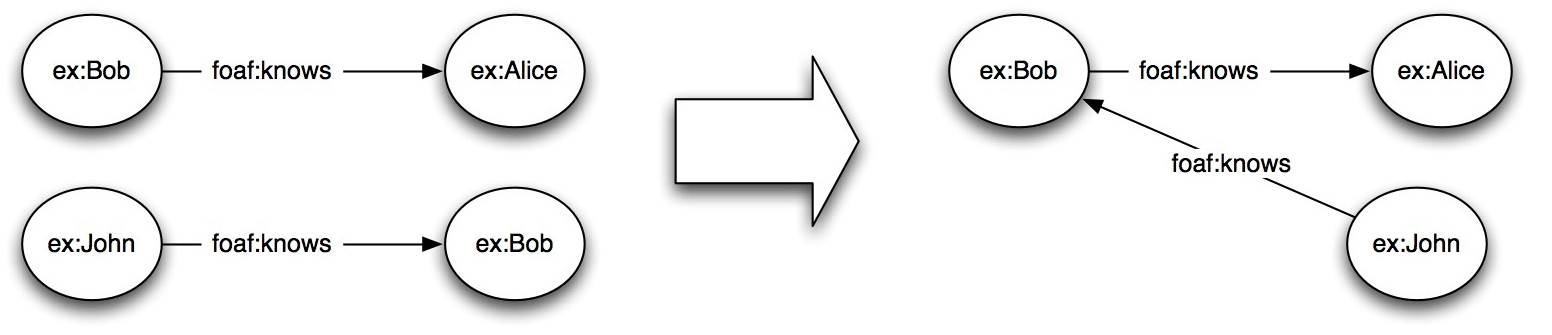
\includegraphics[width=.9\textwidth]{./images/triples1-crop}
\end{figure}

Questo insieme di triple RDF (o grafo) può essere espresso, allo scopo di essere scambiato tra applicazioni e pubblicato sul web, in vari formati di serializzazione.

\clearpage

Ad esempio in RDF/XML:

\begin{lstlisting}
<?xml version="1.0"?>
<rdf:RDF
    xmlns:ex="http://example.org/"
    xmlns:foaf="http://xmlns.com/foaf/0.1//"
    xmlns:rdf="http://www.w3.org/1999/02/22-rdf-syntax-ns#">
    <rdf:Description rdf:about="http://example.org/John">
        <foaf:knows>
            <rdf:Description rdf:about="http://example.org/Bob">
                <foaf:knows rdf:resource="http://example.org/Alice" />
            </rdf:Description>
        </foaf:knows>
    </rdf:Description>
</rdf:RDF>
\end{lstlisting}


La caratteristica più importante di tale modello è l'uso dell'Uniform Resource Identifier (URI). Ciò rende l'impiego di RDF adatto rispetto alla visione Linked Data.

Tornando all’esempio del monumento, supponiamo che i due dataset (amministrazione locale e sovrintendenza) siano stati pubblicati come Linked Data. Per identificare i monumenti, il dataset delle sovrintendenza usa URL (del tipo \emph{http://cultural-heritage-example.org/monument/XYZ}). Il contenuto digitale di tali URL corrisponde alla descrizione dettagliata dei monumenti.
Il data set dell’amministrazione locale, inserendo dei link a tali URL, come avviene in figura 1, permetterebbe a un software di risolvere l’URL e ottenere la descrizione del monumento (sempre aggiornata).

Ancora, dal momento che RDF consente di specificare precisi tipi di risorse, potremmo pensare a un semplice script che trovi tutte le risorse di tipo “monumento” nel dataset dell’amministrazione locale, e che importi, per ciascuna, informazioni aggiuntive, creando così un dataset misto. Su quest’ultimo nuovodata set arricchito, si potrebbero poi fare query del tipo “trova tutti gli alberghi vicini a un monumento successivo al XIII secolo, in cui siano esposte sculture del Canova”.

\floatplacement{figure}{H}
\begin{figure}
\centering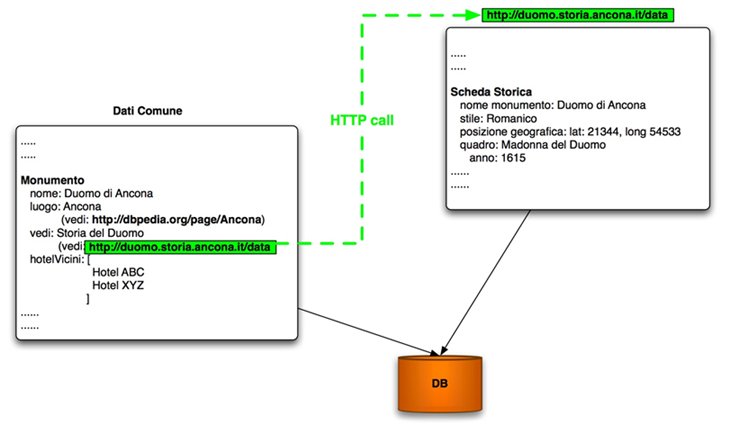
\includegraphics[width=.8\textwidth]{./images/img2}
\end{figure}
Questo esempio è solo uno degli scenari possibili in cui i linked data possono favorire l’interoperabilità tra dataset. Le possibilità sono infinite se pensiamo alla vasta quantità di Linked Open Data già presenti sul Web. \textbf{DBPedia.org}, per esempio, espone una grande porzione di dati di Wikipedia come linked data, mentre \textbf{Geonames} offre descrizioni RDF di entità geografiche. \emph{http://linkeddata.org/} fornisce un quadro dello stato corrente della “Linked data cloud”, e mostra un ecosistema di database interconnessi in rapida crescita.
